

\section*{Introduction}
Après avoir achevé notre étude de l’existant et étudié de près le système actuel, nous abordons l’étape suivante qui consiste à concevoir le nouveau système en utilisant la modélisation UML. L’objectif de cette étape est de déterminer de façon détaillée et précise ce que le nouveau système devrait faire, afin de répondre aux objectifs attendus. Dans ce chapitre nous allons détailler les objectifs fixés du système,en suite nous détaillons ses fonctionnalités et sa logique de fonctionnement. 
%Nous présentons aussi 

 \section{Unified Modeling Language (UML):}
 Dans ce qui suit, nous allons donner une brève description d’UML.
 \subsection{ Définition UML }
 L’OMG définit l’UML comme un langage visuel dédié à la spécification,la construction et la documentation des artéfacts d’un système logiciel. Aussi la façon dont tout le monde modélise non seulement la structure de l’application, le comportement et l’architecture, mais aussi des processus d’affaires et la structure des données. Ce langage est conçu pour modéliser divers types de systèmes et de taille quelconque. Il possède une approche entièrement objet couvrant tout le cycle de développement. Le système est décomposé en un ensemble d’objets collaborant [GUIBERT, 2010].
 
 \subsection{Contenu UML}
 
 L’UML comporte 13 diagrammes qui se répartissent en deux catégories [GUIBERT, 2010]. Nous ne mentionnons que les diagrammes que nous utilisons, les autres sont en annexe G. 
 
 \subsubsection{Diagramme structurel : }
 \begin{itemize}
 \item \textbf{Diagramme de classes (Class Diagram) : }ce diagramme décrit la structure statique du système, il définit les classes, leurs attributs et leurs relations. Il est considéré comme le diagramme le plus important.
  \item  \textbf{Diagramme de paquetages (Package Diagram) : }définit les dépendances entres les paquets (groupement d’éléments UML) constituant un modèle. 
 \end{itemize}
 
 
  \subsubsection{Diagramme comportemental  : }
 
  \begin{itemize}
 	\item \textbf{Diagramme de cas d’utilisation (Use Case Diagram) : } pour décrire les besoins des utilisateurs. 
 	\item  \textbf{Diagramme de séquence(Sequence Diagram):}  décrit comment chaque objet interagit avec l’autre et dans quel ordre, sur un axe temporel donné. Ce diagramme sont associés aux diagrammes de cas d’utilisation.
 	. 
 \end{itemize}



\section{Identification des objectifs}

Au début du projet, nous nous sommes concentrés sur les besoins qui pourraient normalement être considérés comme un système général et nous avons interrogé les ingénieurs de la société nationaux de retraités    "CNR", qui ont exprimé des besoins importants .
 
 
 Nos entretiens ont été complétés en suivant les étapes ci-dessous
 
\textbf{ Étape 1:} Choisir les entretiens Afin d'identifier les besoins, nous avons contacté des personnes pouvant fournir des informations utiles et fournir des explications. Les personnes responsables de la production des différentes unités ou entreprises sont les plus appropriées pour répondre à nos questions.
 
\textbf{Étape 2:}
Planification du développement du programme À ce stade de la planification des entretiens, nous avons étudié deux points essentiels:

- Déterminer le contexte général de l'entretien : "CNR",

- Réglage de la date et de l'heure de l'entretien (date) .

\textbf{ Étape 3:} Préparez-vous pour l’entrevue Préparez les questions de développement et les supports pour un processus sans faille (stylos, cartons de réponses, papiers blancs supplémentaires, clé USB).


\textbf{ Étape 4:} Conduisez l’entretien: Commencez le processus d’entretien en vous présentant d’abord, puis en présentant brièvement notre projet, puis en passant l’entretien en interrogeant la personne concernée et en enrichissant sa conversation d’observations et de questions. Intermédiaire.
 
\textbf{ Étape 5:} Après l'entretien Après avoir pris les informations collectées et conclu l'entretien, nous avons décidé de procéder à d'autres entretiens en développant et en nous réunissant à chaque fois.
 
 
 Sur la base de ces entretiens et de l'entretien avec l'enseignant, nous avons pu identifier les spécifications suivantes:
 
 \subsection{Spécifications fonctionnelles }
 
 \begin{enumerate}
\item  	   Le système doit permettre à l’administrateur  de  Gérer Modale .
\item  	   Le système doit permettre à l’administrateur  de  Gérer Sous-direction .
\item  	   Le système doit permettre à l’administrateur  de Gérer les service.
\item  	   Le système doit permettre à l’administrateur  de Gérer workflow pour les dossier  .
\item  	   Le système doit permettre de  Gérer les tâches des service . 
\item  	   Le système doit permettre à l’administrateur  de Gérer les utilisateur .
\item  	   Le système doit permettre à l’administrateur  de  consulte les historique  et la recherche par tâche .
\item  	   Le système doit permettre à l’administrateur  de  consulte les historique  et la recherche par dossier et les jours pour chaque tâche .
\item  	   Le système doit permettre à l’administrateur  de  consulte bordereau .
\item  	   Le système doit permettre à l’utilisateur   de  Gérer les dossier .
\item  	   Le système doit permettre à l’utilisateur   de  Activé le dossier    .
\item  	   Le système doit permettre à l’utilisateur   de  finir le traitement des dossiers par tâche    .
\item  	   Le système doit permettre à l’utilisateur   de  Gérer les  bordereaux  .
\item  	   Le système doit permettre à l’utilisateur   de  accepte le  bordereau  .
\item  	   Le système doit permettre à l’utilisateur   de  refuse  le  bordereau  .
\item  	   Le système doit permettre à l’utilisateur   de  imprimer le  bordereau  .

 \end{enumerate}
 
 
 
 
  \subsection{Spécifications techniques }
 
 
 
  \begin{enumerate}
 	\item  	   Le système doit être déployé sur le cloud  .
 	\item  	    la configuration et la germanisation de code dynamique . 
 	\item  	  la modélisation de workflow par dessiner  BPMN
 	
 
 	
 \end{enumerate}
 
 
 
 
 
 
 
 
 
 
 
\subsection{ Diagramme de cas d’utilisation }
 
  \subsubsection{ les acteurs de système  }
 
 Un acteur représente l'abstraction d'un rôle joué par des entités externes (utilisateur, dispositif matériel ou autre système) qui interagissent directement avec le système (réception d’information, etc.). Pour notre application,on a trois acteurs : le premier acteur c'est l'administrateur et le deuxième  c'est utilisateur simple  et le troisième c'est l'utilisateur simple .
 
\begin{table}[H]
	\begin{tabular}{|l|l|l|}
		\hline
		\multicolumn{1}{|l|}{Acteur} & Type Acteur & Descriptions \\ \hline
		Utilisateur &  & 2121 \\ \cline{3-3} 
		&  & 1 \\ \cline{3-3} 
		&  &  \\ \cline{3-3} 
		& Acteur Principale &  \\ \cline{3-3} 
		Administrateur &  &  \\ \cline{3-3} 
		&  &  \\ \cline{3-3} 
		&  &  \\ \cline{3-3} 
		&  &  \\ \cline{3-3} 
	\end{tabular}
\end{table}
 
 \subsubsection{ Cas d’utilisation }
 Le diagramme des cas d’utilisation suivant illustre les fonctionnalités qu’un simple utilisateur du système, également l’administrateur, peut faire. Ce diagramme a été inspiré des spécifications citées ci-dessus :
 
 \begin{figure}[H]
 	\centering
 	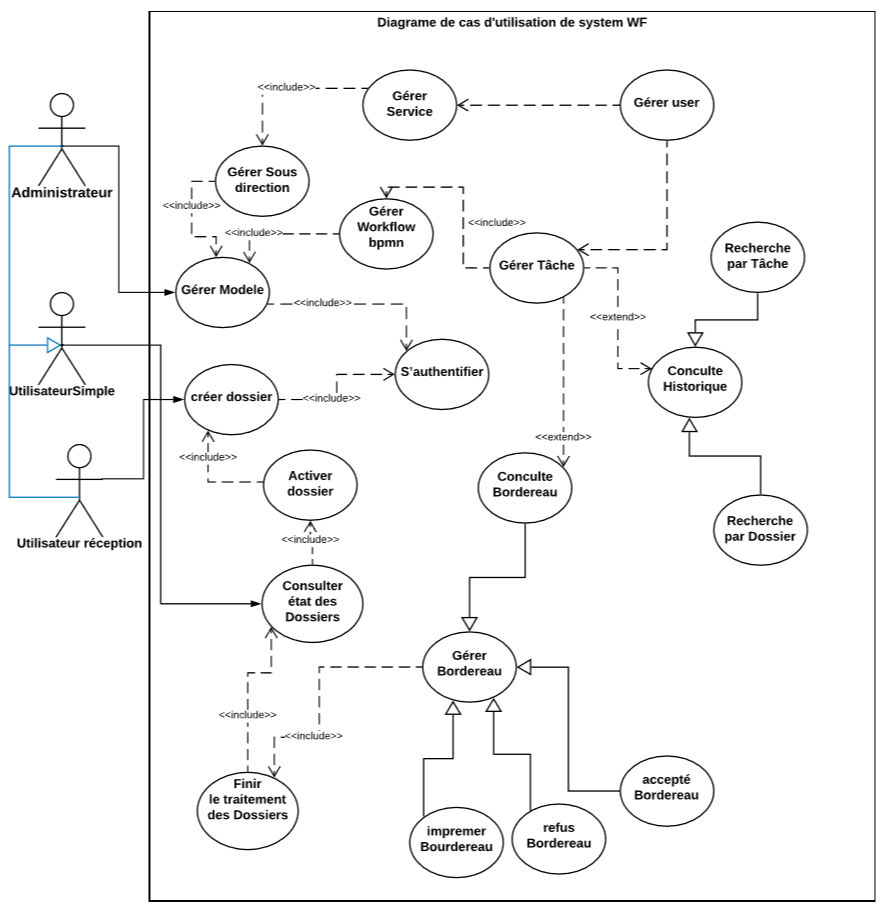
\includegraphics[width=1\linewidth,height=0.6\paperheight
 	]{images/usercase2}
 	\caption{Diagramme de Cas d’utilisation}
 	\label{fig:usercase2}
 \end{figure}
 
 \subsection{ Documentation des cas d’utilisation fonctionnels }
 \subsubsection{ S’authentifier }
 \begin{table}[H]
 	\centering
 	\begin{tabular}{|l|} 
 		\hline
 	\textbf{	CU :} S’authentifier     \\  	\hline
 		\textbf{ID:}1         \\  		\hline
 		\begin{tabular}[c]{@{}l@{}}\textbf{Description brève :} chaque utilisateur doit s’authentifier\\ auprès de l’application afin de pouvoir \\ utiliser les fonctionnalités du système, tel que la consultation du\\ tableau de bord, la manipulation les rapports ...etc. \end{tabular}          \\ 
 		\hline
 		\textbf{Acteurs primaires : }utilisateur, administrateur   \\ 
 		\hline
 		Acteurs secondaires :                                                                                                                                                                                                                                                                                                                                                                                                                                                                                                                                                                                                                                                                                                                                                                             \\ 
 		\hline
 		\begin{tabular}[c]{@{}l@{}}\textbf{Pré-conditions :} – La connexion auprès du serveur d’application doit\\ être réussite. – L’utilisateur \\ doit être enregistré dans le système. \end{tabular}                                                                                                                                                                                                                                                                                                                                                                                                                                                                                                                                                                                                           \\ 
 		\hline
 		\begin{tabular}[c]{@{}l@{}}\textbf{Enchainement principal : }Ce cas d’utilisation commence lorsqu’un\\ utilisateur souhaite accéder à \\ l’application. \\ 1. L’utilisateur saisit le lien de l’application dans barre\\ d’adresse du navigateur. \\ 2. Le serveur répond à l’utilisateur en renvoyant une page\\ d’authentification.\\ 3. L’utilisateur saisit\\ son nom d’utilisateur et son mot de passe et les valide en appuyant sur \\ 4. “Log in”. \\ 5. Le serveur vérifie la validité du nom d’utilisateur et du mot\\ de passe. \\ 6. Le serveur envoie une page d’accueil de l’application à\\ l’utilisateur concerné. \end{tabular}     \\ 
 		\hline
 		Post-conditions : L’utilisateur est connecté.                                                                                     \\ 
 		\hline
 		\begin{tabular}[c]{@{}l@{}}Enchainement alternatif :  \\\begin{tabular}{@{\labelitemi\hspace{\dimexpr\labelsep+0.5\tabcolsep}}l} E1 : La page d’authentification n’apparait pas à l’utilisateur.\end{tabular}\\ * L’enchainement démarre   après le premier point de l’enchainement principal. \\ * Le serveur envoie un message d’erreur à  l’utilisateur. \\\begin{tabular}{@{\labelitemi\hspace{\dimexpr\labelsep+0.5\tabcolsep}}l} E2 : Le nom d’utilisateur ou/et le mot de passe ne sont pas valides.\end{tabular}\\ L’enchainement démarre après le quatrième point de l’enchainement principal. 
 			\\
 			* Le serveur envoie un message d’erreur à l’utilisateur.
 			
 			\\ * Le serveur demande à l’utilisateur de ressaisit le nom d’utilisateur et le mot de passe. \end{tabular}  \\
 		\hline
 	\end{tabular}
 \end{table}
 
  \subsubsection{Créer Dossiers}
 \begin{table}[H]
 	\begin{tabular}{|l|}
 		\hline
 	\textbf{	CU : }Créer   Dossiers \\ \hline
 	\textbf{	ID }: 2 \\ \hline
 	\textbf{	Description brève :} chaque utilisateur pus Créer  et enregistre les noves   Dossiers \\ \hline
 	\textbf{	Acteurs primaires :} utilisateur réception ou initiale, \\ \hline
 		\textbf{Acteurs secondaires :} simple utilisateur \\ \hline
 	\textbf{	Pré-conditions :} L’utilisateur doit être  connecte ou  le système. \\ \hline
 		\begin{tabular}[c]{@{}l@{}}\textbf{Enchainement principal :} Ce cas d’utilisation commence   lorsqu’un utilisateur\\  souhaite accéder à  l’application. \\   1.      L’utilisateur sélectionner de ajouté Nouvo dossier. \\   2.      system répond à l’utilisateur en afficher un formuler de enregistrement.\\   3.       L’utilisateur saisit le   code  et le nom prénom et numéro de typhon\\   de personne de dossier    \\   4.      L’utilisateur vérifier le dossier  et  sélectionner   les chants  présent.\\  en appuyant sur « enregistrer ».\\   5.      Le system envoie une page des dossiers.\end{tabular} \\ \hline
 		\textbf{Post-conditions : }le dossier   est enregistré et ajouté dans le system. \\ \hline
 		\begin{tabular}[c]{@{}l@{}}\textbf{Enchainement alternatif : }    \\  \textbf{ E1:} Le code  de Dossier n’est pas valides ou/et déjà existe.\\   o    L’enchainement démarre après le quatrième point de l’enchainement principal. \\   o     Le serveur envoie un message d’erreur à  l’utilisateur. \\   o   Le serveur demande à l’utilisateur de ressaisit le code de Dossier.\end{tabular} \\ \hline
 	\end{tabular}
 \end{table}
 
 




\subsubsection{Activer Dossiers}
\begin{table}[H]
	\begin{tabular}{|l|}
		\hline
		\textbf{	CU : }Activer Dossiers \\ \hline
		\textbf{	ID }: 3 \\ \hline
		\textbf{	Description brève :}L'utilisateur peut activer le statut du dossier et commencer \\au  début de la tâche "Ajouter au flux de travail" ,\\ après avoir rempli tous les documents.    \\ \hline
		\textbf{	Acteurs primaires :} utilisateur réception ou initiale, \\ \hline
		\textbf{Acteurs secondaires :} simple utilisateur \\ \hline
		\textbf{	Pré-conditions :} Le Dossier  doit être enregistré dans le système.\\ \hline
		\begin{tabular}[c]{@{}l@{}}\textbf{Enchainement principal :} \\ 1.      L’utilisateur sélectionner de ajouté la liste des dossier . \\ 
			2.      system répond à l’utilisateur en afficher  les liste des dossier \\ \{"tous la liste","liste activer ","liste non activer" \} .\\  
			3.       L’utilisateur sélectionner  dossier    \\ 
			4. le system  répond à l’utilisateur en afficher le détaille, est aprés\\  en appuyant sur "Activer". \\  
			5. le system vérifie id "code" de dossier et activer leur état \end{tabular} \\ \hline
		\textbf{Post-conditions : }le dossier  est activé dont la premier tache . \\ \hline
		\begin{tabular}[c]{@{}l@{}}\textbf{Enchainement alternatif : } \end{tabular} \\ \hline
	\end{tabular}
\end{table}





 
 
\subsubsection{Consulter état des Dossiers}
\begin{table}[H]
	\begin{tabular}{|l|}
		\hline
		\textbf{	CU : }Consulter état des Dossiers \\ \hline
		\textbf{	ID }: 4 \\ \hline
		\textbf{	Description brève :}L'utilisateur peut visualiser le statut des dossiers en cours \\ de traitement  en fonction de sa tâche et voir tous les dossiers envoyés par une \\autre tache.     \\ \hline
		\textbf{	Acteurs primaires :} utilisateur  \\ \hline
		\textbf{Acteurs secondaires :}  \\ \hline
		\textbf{	Pré-conditions :} 
		\\ - Le Dossier  doit être Activé dans le système.
		\\ -  L’utilisateur doit être  connecte ou  le système.
		\\ \hline
		\begin{tabular}[c]{@{}l@{}}\textbf{Enchainement principal :} \\ 1.      L’utilisateur sélectionner  le statut des dossiers . \\ 
			2.      system répond à l’utilisateur en afficher  les liste des dossier encore de traitement\\ ou les noves  dossiers envoyés    \end{tabular} \\ \hline
		\textbf{Post-conditions : }L'utilisateur   visualiser le statut  des dossiers par sa tâche. \\ \hline
		\begin{tabular}[c]{@{}l@{}}\textbf{Enchainement alternatif : } \end{tabular} \\ \hline
	\end{tabular}
\end{table}



\subsubsection{Finir le traitement  des Dossiers}
\begin{table}[H]
	\begin{tabular}{|l|}
		\hline
		\textbf{	CU : }Finir le traitement  des Dossier \\ \hline
		\textbf{	ID }: 5 \\ \hline
		\textbf{	Description brève :}L'utilisateur peut sélectionner liste des dossier et finir\\ leur traitement   \\ \hline
		\textbf{ Acteurs primaires :} utilisateur  \\ \hline
		\textbf{Acteurs secondaires :}  \\ \hline
		\textbf{	Pré-conditions :} 
		\\ - Le Dossier  doit être Activé dans    la tâche de l'utilisateur .
		\\ -  L’utilisateur doit être  connecte ou  le système.   
		\\ \hline
		\begin{tabular}[c]{@{}l@{}}\textbf{Enchainement principal :} \\ 1.      L’utilisateur sélectionner la liste  des dossiers pour finir le traitement en payent \\sur "terminer"  , \\ 
			2.      system répond à l’utilisateur et terminer le traitement des dossier par \\ changer état et la date fin de traitement .  \end{tabular} \\ \hline
		\textbf{Post-conditions : }L'utilisateur   finir le traitement   des dossiers par sa tâche. \\ \hline
		\begin{tabular}[c]{@{}l@{}}\textbf{Enchainement alternatif : } \end{tabular} \\ \hline
	\end{tabular}
\end{table}






\subsubsection{Gérer Bordereau}
\begin{table}[H]
	\begin{tabular}{|l|}
		\hline
		\textbf{	CU : }Gérer Bordereau   \\ \hline
		\textbf{	ID }: 6 \\ \hline
		\textbf{	Description brève :}L'utilisateur peut sélectionner liste des dossier et \\Gérer un  Bordereau  \\   \hline
		\textbf{ Acteurs primaires :} utilisateur  \\ \hline
		\textbf{Acteurs secondaires :}  \\ \hline
		\textbf{	Pré-conditions :} 
		\\ - Le Dossier  doit être terminer le traitement  dans    la tâche de l'utilisateur  .
		\\ -  L’utilisateur doit être  connecte ou  le système.   
		\\ \hline
		\begin{tabular}[c]{@{}l@{}}\textbf{Enchainement principal :} \\ 1.      L’utilisateur sélectionner la liste  des dossiers et sélectionner \\le suivant tache  pour transfert    \\ 
			2.  system répond à l’utilisateur et créer  nounous bordereau et afficher la liste\\ de bordereau correspondre a leur tache .
		  \\ 
		3.  L’utilisateur put imprimer et accepte ou refuse le bordereau  .   \end{tabular} \\ \hline
		\textbf{Post-conditions : } L'utilisateur  créer bordereau et transfert les dossier \\si le bordereau accepte par validation d'un utilisateur de la tâche reçu . \\ \hline
		\begin{tabular}[c]{@{}l@{}}\textbf{Enchainement alternatif : }  
	\textbf{	E1:bordereau refuse. }
	\\ * renvoyer a la tâche président tous les dossier   
	
 \end{tabular} \\ \hline
	\end{tabular}
\end{table}
 
 \section{ Représentation des informations }
 \subsection{Diagramme de Classe}
\begin{figure}[H]
	\centering
	\includegraphics[width=1\linewidth]{images/class01}
	\caption{Diagramme de Classe}
	\label{fig:class01}
\end{figure}

  \subsubsection{Conception détaillée} 
Nous allons définir pour chaque classe ses attributs et leur types , ainsi que les méthodes qu’elle offre. Dans le but d’alléger le rapport, nous avons jugé essentiel de ne citer  les classes que nous avons conçu  .
 
 

\subsubsection*{La classe  Sous-Direction}
\begin{table}[H]
  \centering\setlength\tabcolsep{0.8cm}
	\begin{tabular}{|l|l|l|}
		\hline
		\textbf{Attribut}  & \textbf{Type} & \multicolumn{1}{l|}{\textbf{Méthodes}} \\ \hline
	
		id & long & getId() et setId()\\ \cline{1-2}
		nom & String  & getNom() et setNom() \\ \cline{1-2}
	services	& $ List<Service> $ & getServices() et setServices()   \\ \hline
	\end{tabular}
\end{table}
\subsubsection*{La classe Service}
\begin{table}[H]
	\centering
	\begin{tabular}{|l|l|l|}
		\hline
		\textbf{Attribut}  & \textbf{Type} & \multicolumn{1}{l|}{\textbf{Méthodes}} \\ \hline
		
		id & long & getId() et setId()\\ \cline{1-2}
		nom & String  & getNom() et setNom() \\ \cline{1-2}
				sous-Direction & Sous-Direction  & getSous-Direction() et setSous-Direction() \\ \cline{1-2}
		myTasks	& $ List<MyTask> $ & getMyTasks() et setMyTasks()   \\ \hline
	\end{tabular}
\end{table}


\subsubsection*{La classe MyTask}
\begin{table}[H]
	\centering
	\begin{tabular}{|l|l|l|}
		\hline
		\textbf{Attribut}  & \textbf{Type} & \multicolumn{1}{l|}{\textbf{Méthodes}} \\ \hline
		
		id & long & getId() et setId()\\ \cline{1-2}
		nom & String  & getNom() et setNom() \\ \cline{1-2}
			idTask & String & getIdTask() et setIdTask()\\ \cline{1-2}
		services & Service  & getService() et setService() \\ \cline{1-2}
				users	& $ List<User> $ & getUsers() et setUsers()   \\ \cline{1-2}	
				
		nextMyTasks	& $ List<NextMyTask> $ & getNextMyTasks() et setNextMyTasks()   \\ \hline
	\end{tabular}
\end{table}

\subsubsection*{La classe MyTask}
\begin{table}[H]
	\centering
	\begin{tabular}{|l|l|l|}
		\hline
		\textbf{Attribut}  & \textbf{Type} & \multicolumn{1}{l|}{\textbf{Méthodes}} \\ \hline
		
		id & long & getId() et setId()\\ \cline{1-2}
		nom & String  & getNom() et setNom() \\ \cline{1-2}
		idTask & String & getIdTask() et setIdTask()\\ \cline{1-2}
		services & Service  & getService() et setService() \\ \cline{1-2}
		nextMyTasks	& $ List<NextMyTask> $ & getNextMyTask() et setNextMyTask()   \\ \hline
	\end{tabular}
\end{table}

\subsubsection*{La classe NextTask}
\begin{table}[H]
  \centering\setlength\tabcolsep{1cm}

	\begin{tabular}{|l|l|l|}
		\hline
		\textbf{Attribut}  & \textbf{Type} & \multicolumn{1}{l|}{\textbf{Méthodes}} \\ \hline
		
		id & long & getId() et setId()\\ \cline{1-2}
		idTask & String & getIdTask() et setIdTask()\\ \cline{1-2}
		myTask & MyTask  & getMyTask() et setMyTask()   \\ \hline
	\end{tabular}
\end{table}

\subsubsection*{La classe Utilisateur "User"}
\begin{table}[H]
	\centering\setlength\tabcolsep{1cm}
	
	\begin{tabular}{|l|l|l|}
		\hline
		\textbf{Attribut}  & \textbf{Type} & \multicolumn{1}{l|}{\textbf{Méthodes}} \\ \hline
		
		id & long & getId() et setId()\\ \cline{1-2}
		nom & String & getNom() et setNom()\\ \cline{1-2}
			prenom & String & getPrenom() et setPrenom()\\ \cline{1-2}
						tlphon & String & getTlphon() et setTlphon()\\ \cline{1-2}
		myTask & MyTask  & getMyTask() et setMyTask()   \\ \hline
	\end{tabular}
\end{table}




\subsubsection*{La classe Role}
\begin{table}[H]
	\centering\setlength\tabcolsep{1.2cm}
	
	\begin{tabular}{|l|l|l|}
		\hline
		\textbf{Attribut}  & \textbf{Type} & \multicolumn{1}{l|}{\textbf{Méthodes}} \\ \hline
		
		id & long & getId() et setId()\\ \cline{1-2}
		nom & Date() & getNom() et setNom()\\ \hline
	\end{tabular}
\end{table}






\subsubsection*{La classe Dossier}
\begin{table}[H]
	\centering\setlength\tabcolsep{1cm}
	
	\begin{tabular}{|l|l|l|}
		\hline
		\textbf{Attribut}  & \textbf{Type} & \multicolumn{1}{l|}{\textbf{Méthodes}} \\ \hline
		
		id & long & getId() et setId()\\ \cline{1-2}
		nom & String & getNom() et setNom()\\ \cline{1-2}
		prenom & String & getPrenom() et setPrenom()\\ \cline{1-2}
		tlphon & String & getTlphon() et setTlphon()\\ \cline{1-2}
		ch1 & boolean  & getCh1() et setCh1()\\ \cline{1-2}   
				ch2 & boolean  & getCh2() et setCh2() \\ \cline{1-2}
						ch3 & boolean  & getCh3() et setCh3() 
		\\ \hline
	\end{tabular}
\end{table}



\subsubsection*{La classe ListDossier}
\begin{table}[H]
	\centering\setlength\tabcolsep{0.8cm}
	
	\begin{tabular}{|l|l|l|}
		\hline
		\textbf{Attribut}  & \textbf{Type} & \multicolumn{1}{l|}{\textbf{Méthodes}} \\ \hline
		
		id & long & getId() et setId()\\ \cline{1-2}
		bordereau & Bordereau & getBordereau() et setBordereau()\\ \cline{1-2}
		historique & Historique & getHistorique() et setHistorique()\\   \hline
	\end{tabular}
\end{table}


\subsubsection*{La classe Historique}
\begin{table}[H]
	\centering\setlength\tabcolsep{1cm}
	
	\begin{tabular}{|l|l|l|}
		\hline
		\textbf{Attribut}  & \textbf{Type} & \multicolumn{1}{l|}{\textbf{Méthodes}} \\ \hline
		
		id & long & getId() et setId()\\ \cline{1-2}
		dateD & Date() & getDateD() et setDateD()\\ \cline{1-2}
		
				dateF & Date() & getDateF() et setDateF()\\ \cline{1-2}
				
				dossier & Dossier & getDossier() et setDossier()\\ \cline{1-2}
				
					user & User & getUser() et setUser()\\ \cline{1-2}
					
					etat & boolean & isEtat() et setEtat()\\ \cline{1-2}
				transfert & boolean & isTransfert() et setTransfert()\\ \hline
	\end{tabular}
\end{table}
 
   
   \subsubsection*{La classe Bordereau}
   \begin{table}[H]
   	\centering\setlength\tabcolsep{1cm}
   	
   	\begin{tabular}{|l|l|l|}
   		\hline
   		\textbf{Attribut}  & \textbf{Type} & \multicolumn{1}{l|}{\textbf{Méthodes}} \\ \hline
   		
   		id & long & getId() et setId()\\ \cline{1-2}
   		dateD & Date() & getDateD() et setDateD()\\ \cline{1-2}
   	    
   	    user & User & getUser() et setUser()\\ \cline{1-2}
   				myTask1 & MyTask  & getMyTask1() et setMyTask1()   \\ \cline{1-2}
   						myTask2 & MyTask  & getMyTask2() et setMyTask2() \\ \cline{1-2}  
   		etat & String[] & getEtat() et setEtat()\\ \cline{1-2}
		historique & Historique & getHistorique() et setHistorique()\\ \hline
   	\end{tabular}
   \end{table}
\subsection{Diagramme d' activité  }

à partir de cas d'utilisation et de diagramme de classe  va exprimer  le Diagramme d'activité qui  montre interaction des  utilisateurs   en fonction de leurs rôles dans le système en général.
\begin{figure}[H]
	\centering
	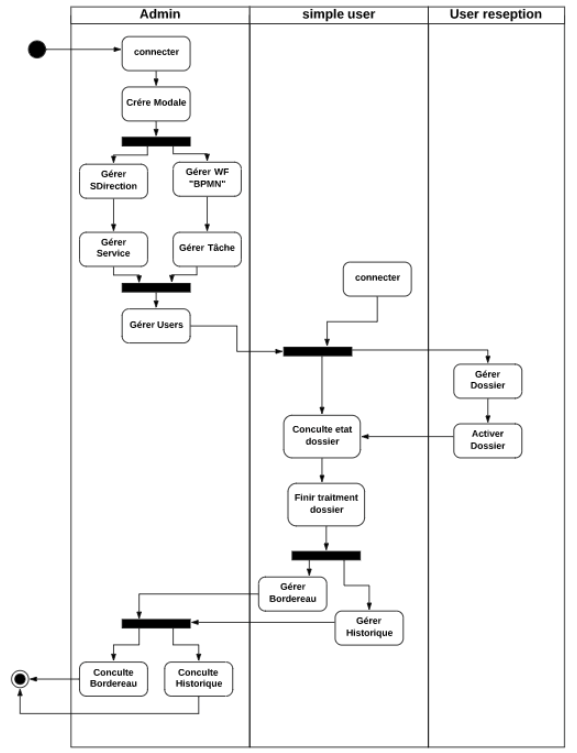
\includegraphics[width=1\linewidth]{images/Dactiviti}
	\caption{Diagramme d'activité qui  montre interaction des  utilisateurs   en fonction de leurs rôles dans le système en général.}
	\label{fig:dactiviti}
\end{figure}



 
   